\section{Implementation and Testing}
	\subsection{Node Implementation}
		The implementation for the protocol has been named Stor, providing the node to handle the back-end protocol communications and the front-end API which serves as an interface to other applications that abstracts details of the network. The UML for the nodes can be found in appendix \ref{uml-node}.
		
		Stor nodes have several management modules that each control different elements of behaviour.
		\subsubsection*{Modules}
		
		\begin{description}[topsep=-5pt,itemsep=-1ex,partopsep=2ex,parsep=1.5ex]
			\item[Connection Module] \hfill \\
				A connections module is provided to handle internodal connections. Any observed node is classed as either active, inactive or unknown. Any newly observed nodes are immediately classed as unknown and will be queued for a test connection to determine their activity status. Should a successful connection be established, the node is reclassified as active, else inactive. The connections module attempts to retain a list of at least 20 active nodes at all times, which can then be used for forwarding and polling of packets. This list is periodically renewed from all nodes known to be active, allowing other nodes to be included in the network. Any active node that cannot be connected to, or fails to respond to a request is reclassified as inactive. Inactive nodes are also randomly tested to check for activity and reclassified appropriately.
			\item[Proof-of-Work Module] \hfill \\
				The proof-of-work module determines which algorithm should be used when generating any proof-of-work. It does this by identifying the nodes any packet will be forwarded to upon insertion and comparing the difficulty required to its own acceptable difficulty. The most common algorithm where the difficulty is not more than $1.5\times$ any accepted difficulty is used for generation. An example of this behaviour is shown in figure \ref{fig:powmodule}.
				%\todo[inline]{Make high-level POW finding diagram}
			\item[Insertion Module] \hfill \\
				To insert some message into the network after the API has applied the relevant function, the packet class is concatenated with the applied message. This structure can then be hashed to produce a checksum that is used in the generation of the proof-of-work. A packet is then made by concatenating the proof-of-work with the applied message. This is forwarded to the connected nodes, and will be further distributed through polling and requesting.
			\item[Retrieval Module] \hfill \\
				A list of packets that should be acquired is kept and the retrieval module works through these looking up any nodes that are known to be in possession of these. Once a node for a desired packet is found, the packet is downloaded from it, checked for validity, and stored.
			\item[Polling Module] \hfill \\
				To determine which packets are stored on other nodes, selective polling is used to enumerate packets and their classes. Each node has a table of nodes and the last time they were polled. This timestamp is passed to the node to be polled in the URL of the HTTP request. Upon a successful poll, the table of packets and which nodes possess them is updated. The node works through the table, looking for broadcast packets that it does not have and attempts to acquire them. Data packets are only obtained through being forwarded to the node, although may also be acquired if referenced by a broadcast.
			\end{description}
			
			\begin{figure}[!hbpt]
				\centering
				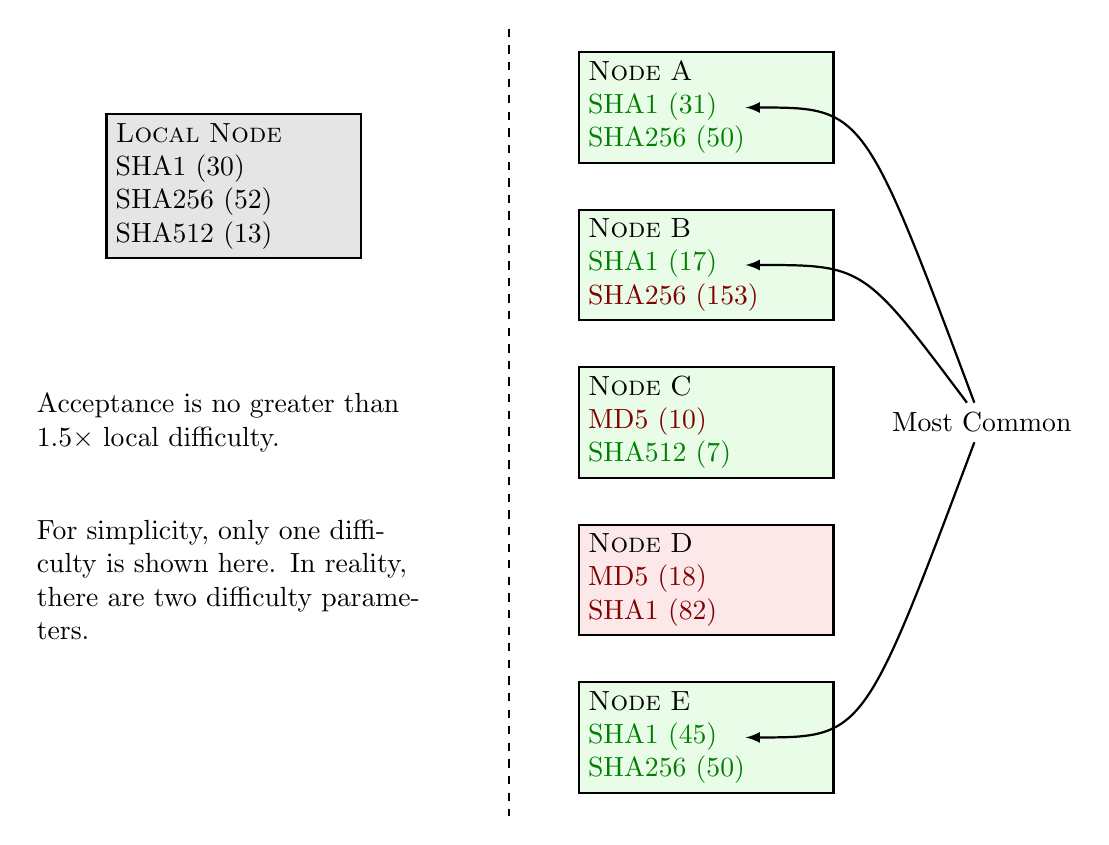
\begin{tikzpicture}[auto, thick]
				
				\node[text width=3cm, draw=black, fill=gray!20] at (-1,3) {\textsc{Local Node}\\SHA1 (30)\\SHA256 (52)\\SHA512 (13)};
				
				\node[text width=5cm] at (-1,0) {Acceptance is no greater than 1.5$\times$ local difficulty.};
				
				\node[text width=5cm] at (-1,-2) {For simplicity, only one difficulty is shown here. In reality, there are two difficulty parameters.};
				
				\node[text width=3cm, draw=black, fill=gray!20!green!10!white] at (5,4) {\textsc{Node A}\\\color{green!50!black}{SHA1 (31)}\\\color{green!50!black}{SHA256 (50)}};
				
				\node[text width=3cm, draw=black, fill=gray!20!green!10!white] at (5,2) {\textsc{Node B}\\\color{green!50!black}{SHA1 (17)}\\\color{red!50!black}{SHA256 (153)}};
				
				\node[text width=3cm, draw=black, fill=gray!20!green!10!white] at (5,0) {\textsc{Node C}\\\color{red!50!black}{MD5 (10)}\\\color{green!50!black}{SHA512 (7)}};
				
				\node[text width=3cm, draw=black, fill=gray!20!red!10!white] at (5,-2) {\textsc{Node D}\\\color{red!50!black}{MD5 (18)}\\\color{red!50!black}{SHA1 (82)}};
				
				\node[text width=3cm, draw=black, fill=gray!20!green!10!white] at (5,-4) {\textsc{Node E}\\\color{green!50!black}{SHA1 (45)}\\\color{green!50!black}{SHA256 (50)}};
				
				\draw[thick, dashed, black] (2.5,5) -- (2.5,-5);
				
				\node[] (common) at (8.5,0) {Most Common};
				
				\draw[latex-, thick, black] (5.5,-4) .. controls (7,-4) .. (common);
				
				\draw[latex-, thick, black] (5.5,2) .. controls (7,2) .. (common);
				
				\draw[latex-, thick, black] (5.5,4) .. controls (7,4) .. (common);
				
				\end{tikzpicture}	
				
				\caption{Example showing the effect of local proof-of-work difficulty on node selection}
				\label{fig:powmodule}
				%\end{center}
			\end{figure}
			
		\subsubsection*{RESTful Interface}
			Nodal communications support a RESTful interface using HTTP for transfers. Each node will be accessible through a GET request to the following pages:
			\begin{description}[topsep=-5pt,itemsep=-1ex,partopsep=2ex,parsep=1.5ex]
				\item[/] Information Page \\ Displays supported proof-of-work algorithms and their associated difficulty.
				\item[/poll/\textit{timestamp}] Packet Polling Page \\ Displays the packets stored and their class.
				\item[/nodes] Nodes Page \\ Displays the nodes that are known to be active.
				\item[/data/\textit{packetHash}] Packet Download \\ Downloads the specified packet.
			\end{description}
			
			POST requests to /data are allow allowable, enabling packet forwarding.
	
			Communications require the serialisation of some data structures to pass them between nodes. As different serialisation techniques have differing advantages and disadvantages, enforcing all nodes to support just a single technique was deemed a poor choice. Rather, any serialisation technique can be supported if later implemented. To determine the technique to use, the HTTP \textit{Accept} header is used, enumerating the types of data that the requester is willing to accept. Any common technique between the 2 nodes is used. Should there be no common techniques, a HTTP \textit{Unacceptable} error code is set.
			
			%While HTTP and JSON offer wide support, they each carry large overheads. Because of this, communications are not as efficient as they could be. While Stor nodes only accept HTTP connections, because different serialisation techniques can be added at a later date, this is
	
		\subsubsection*{Persistence}
			HSQLDB, an embedded database, is used to provide persistence across executions. HSQLDB allows local storage without the running a daemon and hence requiring no setup from the user. Nodal activity observations will be kept in an attempt to determine which nodes are likely to be active on startup, giving quick access to the network. Records of when nodes were lasted polled are also stored in order to assist in saving resources. Any packets help also persist to increase availability.
			
			Ideally, any data held as part of the persistence would be stored encrypted to prevent an adversary with disk access from determining any prior usage. HSQLDB provides database encryption, which uses a user-supplied password on node startup, if desired. Unfortunately, the encryption method used is somewhat weak in that patterns can be determined in the database, such as fields that contain the same values. While not ideal, HSQLDB's built-in encryption has been used to provide some protection.
		\subsubsection*{Hashes and Proof-of-Works}
			Hashing algorithms have quite a history of becoming dangerously obsolete. As such, it was felt that supporting multiple hashing algorithms was a wise decision in comparison to forcing a single algorithm upon all applications. Stor currently allows all algorithms that come with the standard Java cryptography provider, although adding more in the future is easily done. 
		
			Like hashing algorithms, nodes also support multiple proof-of-work algorithms, allowing for future flexibility. Each node has a collection of acceptable proof-of-work algorithms along with the relevant difficulty parameters. These difficulty parameters consist of a constant and coefficient term, allowing the difficulty to by computed by equation \ref{eq:difficulty}. 
		
			\begin{equation} \label{eq:difficulty}
			\text{difficulty} = \text{constant} + \text{size} \times \text{period} \times \text{coefficient}
			\end{equation}
			
			Proof-of-work algorithms, such as that described in Hashcash, use an exponential approach in order to achieve difficulty. In Hashcash, the difficulty is equal to the number of nibbles\footnote{A nibble is equivalent to half a byte.} at the start of the proof-of-work checksum that are zero, and hence the amount of work required as a function of the difficulty size is exponential. This exponential nature is well-suited for systems that require a change in difficulty over time, where computing power is also expected to be exponential. For Stor, this does not follow, as the difficulty needs to be more flexible, and the amount of work to produce a proof-of-work should ideally be linear with respect to difficulty. To achieve this, the difficulty, which can take the form of any natural number, is transformed to a number in some finite interval with equation \ref{eq:transdif}. The proof-of-work is valid if the relevant proof-of-work checksum is less than or equal to this transformed difficulty (equation \ref{eq:difdif}).
		
			\begin{equation} \label{eq:transdif}
			\text{difficulty}' = M - \frac{\text{difficulty}}{M}
			\qquad\parbox{4.0cm}{\footnotesize$\begin{aligned} M &= \text{ maximum}\end{aligned}$}
			\end{equation}
			
			\begin{equation} \label{eq:difdif}
			\text{Hash}(checksum, period, size, nonce) \le \text{difficulty}'
			\end{equation}

			\begin{figure}[h!]
	\begin{center}
		\begin{tikzpicture}
		\begin{axis}[
			width=0.8\linewidth, % Scale the plot to \linewidth
			height=0.6\linewidth,
			grid=major, % Display a grid
			grid style={dashed,gray!30}, % Set the style
			xlabel=Difficulty,
			ylabel=Number of search iterations,
			xmin=0, xmax=100000, xtick={0},
			ymin=0, ymax=6000, ytick=0,
			axis lines=left,
			scaled ticks=false,
		]
		\addplot[scatter,
		only marks,]
		table[x=column 1,y=column 2,col sep=comma] {step-pow.csv}; 
		\end{axis}
		\end{tikzpicture}
		\caption{Step POW}
		\label{fig:steppow}
	\end{center}
\end{figure}

\begin{figure}[h!]
	\begin{center}
		\begin{tikzpicture}
		\begin{axis}[
		width=0.8\linewidth, % Scale the plot to \linewidth
		height=0.6\linewidth,
		grid=major, % Display a grid
		grid style={dashed,gray!30}, % Set the style
		xlabel=Difficulty,
		ylabel=Number of search iterations,
		xmin=0, xmax=10000, xtick={0},
		ymin=0, ymax=25000, ytick=0,
		axis lines=left,
		scaled ticks=false,
		]
		\addplot[scatter,
		only marks,]
		table[x=column 1,y=column 2,col sep=comma] {lin-pow.csv}; 
		\end{axis}
		\end{tikzpicture}
		\caption{Linear POW}
		\label{fig:linpow}
	\end{center}
\end{figure}	
		
		\subsubsection*{Packets}
			The packets are as described in the protocol, but no specific implementation of the meta packet is used.
			
			Both data and broadcast packets are equipped with class flags, allowing the class of a packet to be determined from a single field. In a data packet, this has been selected to be the byte \textit{0xDA}, while with broadcasts, it is \textit{0xBC}. The proof-of-work uses the hash of the class flag concatenated with the payload for validity. Each packet has a unique identifier, which serves as a hash of the entire packet, including the proof-of-work header. Figures \ref{fig:datapacket} and \ref{fig:broadcastpacket} show the high-level structures of the data and broadcast packet.
 			
			\begin{figure}
				\centering
				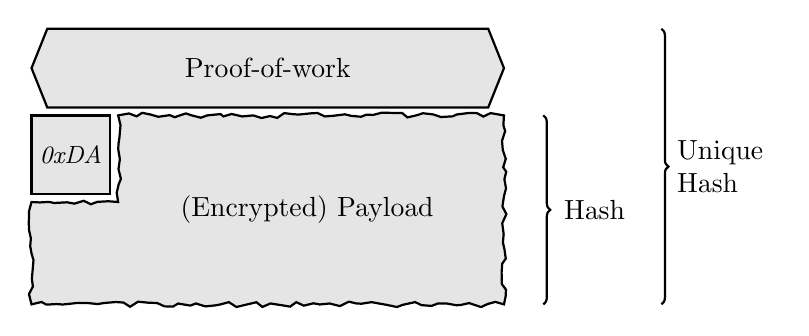
\begin{tikzpicture}[auto, thick]
				\draw [fill=gray!20, draw=black](0,0) -- (0.2,0.5) -- (5.8,0.5) -- (6,0) -- (5.8,-0.5) -- (0.2,-0.5) -- cycle;
				\draw [fill=gray!20, draw=black](0,-0.6) -- (1,-0.6) -- (1,-1.6) -- (0,-1.6) -- cycle;
				\draw [fill=gray!20, draw=black, decorate, decoration={random steps,segment length=3pt,amplitude=1pt}](1.1,-0.6) -- (6,-0.6) -- (6,-3) -- (0,-3) -- (0,-1.7) -- (1.1,-1.7) -- cycle;
				\node at (3,0) {Proof-of-work};
				\node at (0.5, -1.1) {\small{\textit{0xDA}}};
				\node at (3.5, -1.8) {(Encrypted) Payload};
				
				\draw [draw=black, decorate,decoration=brace] (6.5,-0.6) -- (6.5,-3);
				\node at (7.15, -1.8) {Hash};
				
				\draw [draw=black, decorate,decoration=brace] (8,0.5) -- (8,-3);
				\node[text width=1.2cm] at (8.8, -1.25) {Unique Hash};
				\end{tikzpicture}	
				
				\caption{High-level data packet structure example showing \textit{0xDA} class flag}
				\label{fig:datapacket}
				%\end{center}
			\end{figure}
			
			\begin{figure}
				\centering
				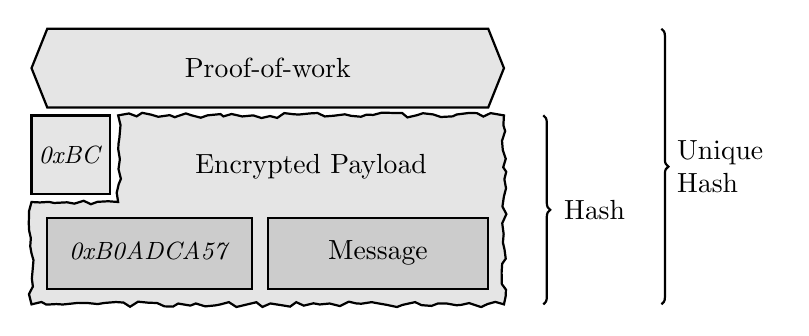
\begin{tikzpicture}[auto, thick]
				\draw [fill=gray!20, draw=black](0,0) -- (0.2,0.5) -- (5.8,0.5) -- (6,0) -- (5.8,-0.5) -- (0.2,-0.5) -- cycle;
				\draw [fill=gray!20, draw=black](0,-0.6) -- (1,-0.6) -- (1,-1.6) -- (0,-1.6) -- cycle;
				\draw [fill=gray!20, draw=black, decorate, decoration={random steps,segment length=3pt,amplitude=1pt}](1.1,-0.6) -- (6,-0.6) -- (6,-3) -- (0,-3) -- (0,-1.7) -- (1.1,-1.7) -- cycle;
				\node at (3,0) {Proof-of-work};
				\node at (0.5, -1.1) {\small{\textit{0xBC}}};
				\node at (3.55, -1.25) {Encrypted Payload};
				
				\draw [fill=gray!40, draw=black](0.2,-1.9) -- (2.8,-1.9) -- (2.8,-2.8) -- (0.2,-2.8) -- cycle;
				\node at (1.5,-2.35) {\small{\textit{0xB0ADCA57}}};
				
				\draw [fill=gray!40, draw=black](3,-1.9) -- (5.8,-1.9) -- (5.8,-2.8) -- (3,-2.8) -- cycle;
				\node at (4.4,-2.35) {Message};
				
				\draw [draw=black, decorate,decoration=brace] (6.5,-0.6) -- (6.5,-3);
				\node at (7.15, -1.8) {Hash};
				
				\draw [draw=black, decorate,decoration=brace] (8,0.5) -- (8,-3);
				\node[text width=1.2cm] at (8.8, -1.25) {Unique Hash};
				\end{tikzpicture}	
				
				\caption{High-level broadcast packet structure example showing \textit{0xBC} class flag and \textit{0xB0ADCA57} decryption magic number}
				\label{fig:broadcastpacket}
				%\end{center}
			\end{figure}
		
		\subsubsection*{Security}
			Care has been taken to prevent leakage of sensitive information, such as anything could be used to help determine the geographical location of a node. For instance, HTTP headers often contain a Date field which also contains time zone information. As part of the HTTP standard, this is always GMT, so does not require special attention. However, as timestamps are used elsewhere in the application for the packet validity periods, care has been taken to ensure that these all follow the same time zone, GMT. In addition to time zone leakage, versioning leakage has been avoided by not advertising any version number.
			
			While the node implementation offers some cryptographic method; no ciphers, padding or hashing algorithms have been invented or implemented. Rather, existing, trusted implementations have been used. Considerations were made for the legality around the export of a product containing cryptography and later determined that as long as all cryptography was linked externally from the application, no export license was required. As such, Java's standard cryptography provider has been used, although Bouncycastle was also considered as it offers a wider and freer range of algorithms.
			
			In several instances, there has been a desire to apply serialisation to polymorphism, therefore allowing the subclasses of some supertype to be serialised and deserialsed transparently. While this could have been implemented in order to achieve a more elegant structure to the code in some areas, such as the \texttt{ProofOfWork} class, polymorphic serialisation requires the construction of arbitrary objects, and if done incorrectly, presents a high potential for vulnerabilities. In fact, this is the exact reason as to why polymorphic serialisation is not supported by the GSON library by default.
			
		\subsubsection*{Tor Interface}
			The interface to Tor was the first element to be implemented due to the importance of its role in the project.
			
			This module communicates with a Tor instance in order to create hidden services programmatically. Bundling a Tor instance with Stor nodes was considered, but given the complications regarding keeping the instance up to date with the latest Tor releases when included in a package and potential conflicts arising from running multiple instances on a single system, it was decided that responsibility of running an instance should be delegated beyond the API for now.
			
			Tor provides an option to enable a control port, allowing the post-startup configuration. This control port is only bound locally and can use authentication to ensure any connections are legitimate. This interface module uses the Tor controller from \texttt{net.freehaven.tor.control} to connect the control port of a Tor instance. The module allows for password authentication with the control port using the password in the \textit{stor.cfg} configuration file.
		\subsubsection*{API}
			The API starts an instance of a Stor node and when commanded to receive a packet, will create a hook for a private identity, which is hooked into the broadcast feed, allowing it to process all broadcast packets.
			
			The API contains abstract classes \texttt{PublicIdentity} and \texttt{PrivateIdentity}, which require implementations of the function to apply and inverse. This abstraction makes it easy to provide alternative identities with custom representations and cryptography. It is hoped that through this abstraction, it may in fact be possible to directly hook an application's existing identity scheme straight into Stor's API. For basic usability, an implementation has been provided, using protocol buffers for data representation and RSA/ECB/PKCS1 for the cryptography.
			
			The sending of fake packets to add to anonymity has not been implemented in the node, but rather, has been left as a usage detail, where some applications may not desire this (due to added resource costs). Using this feature from the API is as simple as inserting some random payload with a valid proof-of-work header.
		%\subsection{Attacks and Mitigations}
		%	\subsubsection*{Packet Class Poison Attack}
		%	\subsubsection*{Fake Pseudoidentity Attack}
		\subsection{Licensing}
			As one of the core aims of the project is to release the code for Stor and its API under a BSD license, software licensing must be taken into account to not only ensure that anyone wishing to use the code can do so, but also to ensure that any third party code used is licensed to allow its use within this project.
		\subsubsection*{External Libraries}
			\begin{description}[topsep=-5pt,itemsep=-1ex,partopsep=2ex,parsep=1.5ex]
				\item[\texttt{net.freehaven.tor.control}]\textbf{\hfill BSD License} \\
					Provides a high-level interface for communicating with Tor's control port.
				\item[\texttt{org.eclipse.jetty}]\textbf{\hfill Apache 2.0 and Eclipse Public License} \\
					An embedded webserver that allows delegation of request handling.
				\item[\texttt{org.apache.commons}]\textbf{\hfill Apache 2.0 License} \\
					Provides various collections and utility classes.
				\item[\texttt{com.google.code.mimeparse}]\textbf{\hfill MIT License} \\
					A utility for parsing mime types for HTTP request acceptance.
				\item[]\hspace*{-1ex}\textbf{\texttt{tinfoil}\footnote{\texttt{tinfoil} does not provide a fully qualified package name.} (for \texttt{TorLib}) \hfill MIT License}\\
					Provides a method for performing .onion address resolution.
				\item[\texttt{com.google.gson}]\textbf{\hfill Apache 2.0 License}\\
					Provides serialisation/deserialisation for JSON.
				\item[\texttt{org.hsqldb}]\textbf{\hfill BSD License}\\
					An embedded SQL database that provides encrypted data persistence.
				\item[\texttt{com.google.protobuf}]\textbf{\hfill BSD License}\\
					A high-efficiency data structure serialiser.
			\end{description}
	\subsection{Demonstration}
		To demonstrate the API in action, two applications have been created. Application A, the sender, knows the public identity of application B, and once the API has started the node, prompts for an input which is fed into the API and inserted into the network for B to discover, retrieve and display to the user.
		
		Under most conditions, the demonstration startup time is around 20 seconds, with the message latency after a completed proof-of-work is around a second. In some rare cases, Tor network conditions cause a startup time of up to 20 minutes, although this is the time to get the hidden service descriptor to propagate, and is a one-time cost, not required for additional startups.
	\subsection{Testing}
		JUnit tests have been utilised to provide automated unit testing for individual components of the system, taking into account the internal workings of these elements. These have come in the form of both fine-grained and coarse-grained tests. Some of these tests are shown in appendix \ref{sec:unit-tests}.
	
		Difficulties with testing encryption were met when building unit tests because all encryption performed as part of Stor uses some form of padding or initialisation vectors, creating a different ciphertext on each execution. Because of this, the assumption that the cryptography provider used is working as expected is made, although tests where some known value is encrypted then decrypted are performed to test code logic.
		
		As Stor is highly interactive through interfacing with the API, Tor and other Stor nodes, some elements are difficult to automatically test. Testing these elements has been achieved through manual usability tests. These tests focus on the usability and overall functionality of the system, and have been performed at distinct points through the development. These tests are shown in appendix \ref{sec:usability-tests}.
		
		As part of the Stor startup process, self-tests are performed to ensure that some modules are working as expected. This is true for critical elements that can not under normal operation fail such as the database, webserver, Tor interface and serialiser. Perhaps the most exposed example of this is the test where a node will check that it's hidden service is publicly accessible by performing a connection to itself.
		
		\subsubsection*{Leakage of .onion Addresses}
			During testing, it was discovered that metadata was leaking through the form of hidden service DNS requests. This kind of problem is described in \cite{Thomas:2014:MLO:2665943.2665951}, where it is shown to be quite a widespread issue. For Stor, the leakage occurred because when using \texttt{URLConnection}s, Java does not use any specified SOCKS proxy for address resolution, hence having the potential to leak information about which nodes are being connected to under some conditions.
			
			To resolve this, hidden service address resolution is handled separately to the proxy. The responsibility for this is partially handled by \texttt{tinfoil.TorLib}, allowing Stor to pass a hidden service address to tor's resolver, which returns a local IP address that can then be used to make connections to the hidden service in the future without having to specify the hidden service address. This method ensures that no leakage occurs.